% =====================================================================
\clearpage
\partieENO{Les plantes et les essais}

La tour n'a de sens que si elle fait pousser des plantes. Cette partie présente la plante que j'ai choisie pour commencer, la laitue, et ce que j'ai déjà observé. Je commence par les valeurs cibles de la laitue, puis par la conversion de l'EC en ppm, puis par les premiers semis avec leurs photos. Je termine par le calendrier prévu et la façon dont je suivrai la croissance.

\Needspace{8\baselineskip}\subsection{Les besoins de la laitue}

J'ai choisi la laitue pour débuter, parce qu'elle pousse vite (environ 32 jours après le repiquage) et qu'elle supporte bien l'hydroponie. Elle est cultivée en NFT (film d'eau) dans les études que j'ai trouvées, un système proche de ma tour. Le tableau donne les valeurs retenues dans le dashboard, par stade de croissance. Les jours sont comptés à partir de la mise en tour du plant.

\begin{table}[H]
\centering
\small
\begin{tabular}{|l|c|c|c|}
\hline
\textbf{Stade} & \textbf{Jours} & \textbf{EC cible (\unit{\micro S/cm})} & \textbf{pH cible} \\
\hline
Reprise & 0 à 5 & 1000 à 1200 & 5,6 à 6,0 \\
\hline
Croissance des feuilles & 5 à 22 & 1200 à 1600 & 5,6 à 6,0 \\
\hline
Pommaison & 22 à 32 & 1400 à 1800 & 5,6 à 6,0 \\
\hline
Prête à récolter & 32 et plus & 1400 à 1800 & 5,6 à 6,0 \\
\hline
\end{tabular}
\caption{Valeurs cibles de la laitue (recherche documentaire du 31 octobre 2026).}
\end{table}

Les alarmes du dashboard se déclenchent si l'EC sort de \qtyrange{800}{2200}{\micro S/cm} ou si le pH sort de 5,2 à 6,5. Au-dessus d'environ \qty{2200}{\micro S/cm}, la laitue risque des pointes de feuilles brûlées et un goût amer. L'eau idéale est entre \qty{18}{\celsius} et \qty{22}{\celsius}. La partie 6 montre que cette plage sera difficile à tenir à Tahiti : c'est un point à surveiller dès les premiers essais.

Pour la tomate cerise et le poivron, les plages sont plus élevées (EC jusqu'à \qty{2800}{\micro S/cm} pour la tomate en fructification) et leur culture est plus longue (60 à 75 jours avant la récolte). Elles sont enregistrées dans le dashboard, mais je ne les essaie qu'après la laitue.

\naturecalc{théorie (formule démontrée, valeurs de fiches techniques et hypothèses ; rien de mesuré)}
\begin{demonstration}[conversion de l'EC en ppm]
\resultat{\mathrm{ppm} = f \times EC}
Je note $EC$ la conductivité, en $\mu$S/cm, et $f$ un facteur de conversion sans unité qui dépend de l'échelle. Les appareils du commerce estiment la masse de sels dissous (en ppm, c'est-à-dire en mg/L) en multipliant la conductivité par un facteur : $f = 0{,}5$ pour l'échelle 500, $f = 0{,}7$ pour l'échelle 700. Pour la cible de croissance de la laitue, $EC = \qty{1400}{\micro S/cm}$ :
\begin{align*}
\mathrm{ppm}_{500} &= 0{,}5 \times \qty{1400}{\micro S/cm} = \qty{700}{ppm}\\
\mathrm{ppm}_{700} &= 0{,}7 \times \qty{1400}{\micro S/cm} = \qty{980}{ppm}
\end{align*}
La conversion dépend de l'échelle : je donne donc toujours l'EC en $\mu$S/cm, qui est la grandeur mesurée.
\end{demonstration}

\Needspace{8\baselineskip}\subsection{Les premiers semis}

J'ai semé les premières laitues le \qty{27}{octobre}. Elles poussent, sans eau nutritive pour l'instant, sous la seule lumière d'une fenêtre. Elles mesuraient environ \qty{5}{cm} le 11 novembre, soit 15 jours après le semis. Les photos montrent les plants dans la mousse de germination.

\begin{figure}[H]
\centering
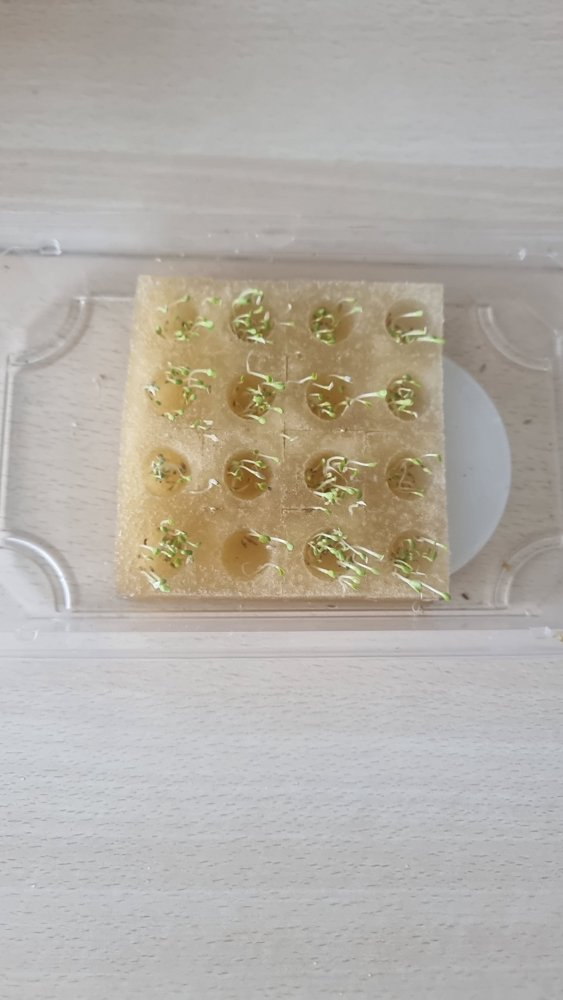
\includegraphics[height=6.2cm]{img/germ_haut2.jpg}\hfill
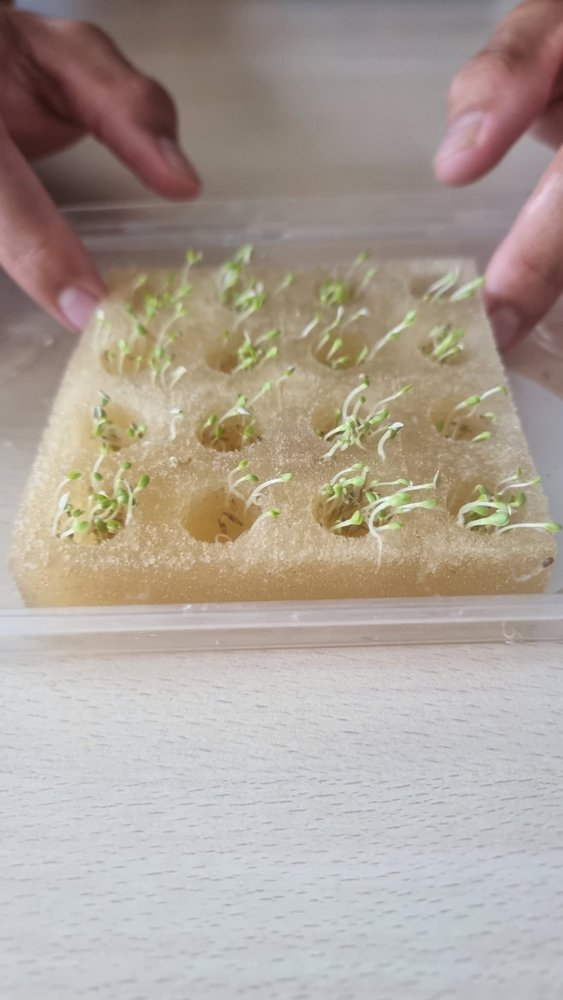
\includegraphics[height=6.2cm]{img/germ_main.jpg}\hfill
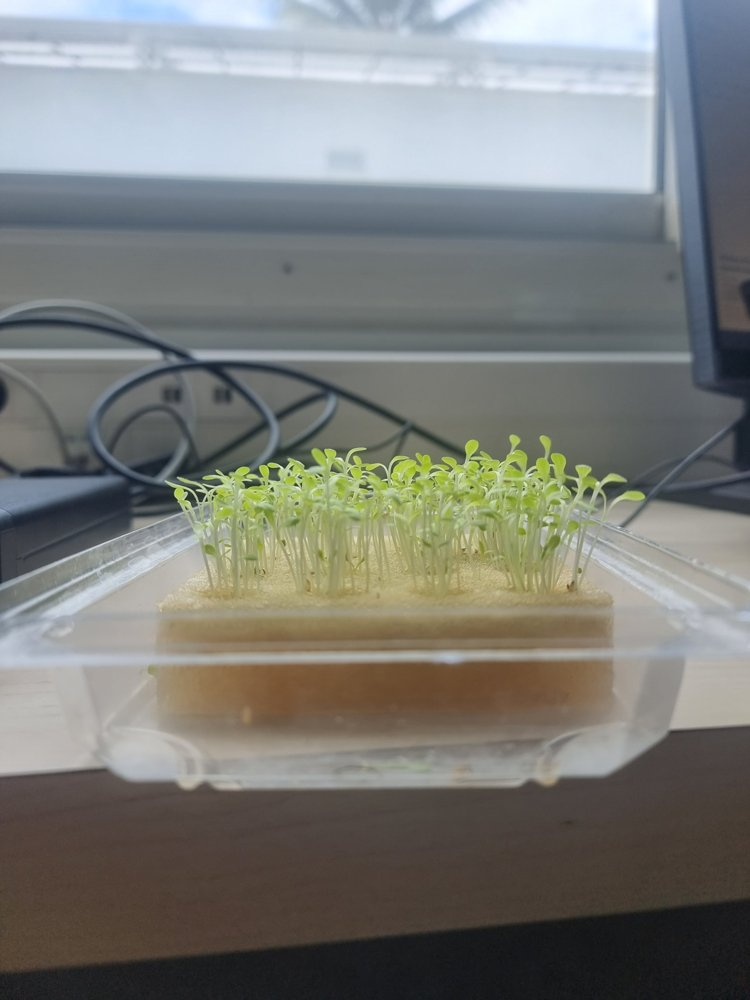
\includegraphics[height=6.2cm]{img/germ_cote.jpg}
\caption{Les semis de laitue dans la mousse de germination : vue de dessus, plants tenus à la main, vue de côté.}
\end{figure}

\Needspace{8\baselineskip}\subsection{Le calendrier prévu et le suivi}

D'après la recherche documentaire, le passage du semis au repiquage dure environ 18 jours pour la laitue, et la pleine maturité arrive vers le jour 32 après la mise en tour.

\naturecalc{prévision, à partir de la date de semis observée (27 octobre) et de durées tirées de la littérature}
\begin{demonstration}[dates prévues]
\resultat{\text{récolte} \approx 16\ \text{décembre 2026}}
Je note $d_s$ la date du semis, $d_r$ celle de la mise en tour et $d_h$ celle de la récolte. Le repiquage a lieu 18 jours après le semis, la récolte 32 jours après le repiquage :
\begin{align*}
d_r &= d_s + \qty{18}{j} = \text{27 octobre} + \qty{18}{j}\\
d_r &= \text{14 novembre}
\end{align*}
\begin{align*}
d_h &= d_r + \qty{32}{j} = \text{14 novembre} + \qty{32}{j}
\end{align*}
Du 14 au 30 novembre, il y a 16 jours ; il en reste $32 - 16 = 16$ en décembre :
\begin{align*}
d_h &= \text{16 décembre 2026}
\end{align*}
La fourchette de la littérature (25 à 45 jours après le repiquage) donne une récolte entre le 9 décembre 2026 et le 29 décembre 2026.
\end{demonstration}

Pour le suivi, je compterai chaque semaine le nombre de plants vivants, je mesurerai la hauteur de trois plants repères avec une règle et je photographierai la tour du même endroit. Je noterai aussi la date de passage à l'eau nutritive, la température de l'eau et les corrections de dosage faites par le Pi. À la récolte, je pèserai les 12 laitues pour connaître le rendement réel, que j'utilise dans l'étude financière.

\begin{aretenir}
La laitue demande un pH de 5,6 à 6,0 et une EC de 1200 à \qty{1600}{\micro S/cm} en croissance. Les premières sont semées depuis le 27 octobre et mesurent environ \qty{5}{cm} au 11 novembre. La récolte est attendue vers le 16 décembre, sous réserve du passage à l'eau nutritive et de la température de l'eau.
\end{aretenir}

